\documentclass[11pt]{article}
\usepackage[utf8]{inputenc}
\usepackage[T1]{fontenc}
\usepackage[spanish]{babel}
\usepackage{amsmath, amssymb, amsthm}
\usepackage{braket}
\usepackage{graphicx}
\usepackage[margin=2.5cm]{geometry}
\usepackage{hyperref}

\allowdisplaybreaks

\newcommand{\ii}{\mathrm{i}}
\newcommand{\ee}{\mathrm{e}}
\newcommand{\dd}{\mathrm{d}}
\newcommand{\adag}{\hat a^\dagger}
\newcommand{\Real}{\operatorname{Re}}
\newcommand{\Imag}{\operatorname{Im}}

\title{Estados apachurrados}
\author{Ricardo Del Rosal Gardu\~no \\ \small Doctorado en F\'isica, BUAP}
\date{Notas a partir de Schleich, \emph{Quantum Optics in Phase Space}}

\begin{document}
\maketitle

\section{Motivaci\'on f\'isica}

Los estados apachurrados, o \emph{squeezed states}, aparecen cuando se cambia
la anchura de las fluctuaciones cu\'anticas de un oscilador sin violar el
principio de incertidumbre. En los estados coherentes, las incertidumbres de
posici\'on y momento son iguales, y su producto toma el valor m\'inimo
$\hbar/2$. En un estado apachurrado el producto sigue siendo m\'inimo, pero
las incertidumbres ya no est\'an repartidas sim\'etricamente: una cuadratura se
vuelve m\'as precisa y la conjugada se vuelve m\'as ruidosa.

Una manera f\'isica de producir esta redistribuci\'on es cambiar
repentinamente la frecuencia del oscilador. Si el potencial se hace m\'as
estrecho, el estado que antes era el vac\'io ya no coincide con el nuevo
vac\'io, sino que se ve apachurrado respecto al oscilador original. Esta idea
puede formularse de manera equivalente con el operador de apachurramiento
$\hat S(s)$.

En estas notas se usa un par\'ametro real positivo $s>0$. Para $s=1$ no hay
apachurramiento. Para $s>1$ la distribuci\'on en posici\'on se estrecha y la de
momento se ensancha. Para $s<1$ ocurre lo contrario.

\section{Estado base y cambio repentino de frecuencia}

Se parte del estado base del oscilador arm\'onico. Su funci\'on de onda en
posici\'on es
\begin{equation}
  u_0(x)
  =
  \left(\frac{K^2}{\pi}\right)^{1/4}
  \ee^{-K^2x^2/2},
  \qquad
  K=\sqrt{\frac{M\Omega}{\hbar}}.
\end{equation}
Aqu\'i $\Omega$ es la frecuencia del oscilador. Si se realiza un cambio
repentino
\begin{equation}
  \Omega\longrightarrow \frac{\Omega}{s},
  \qquad s>0,
\end{equation}
entonces el nuevo par\'ametro de anchura es
\begin{equation}
  K'=\sqrt{\frac{M(\Omega/s)}{\hbar}}
  =
  \frac{K}{\sqrt{s}}.
\end{equation}
Como $K^2=sK'^2$, el estado base original puede reescribirse en t\'erminos de
$K'$ como
\begin{equation}
  u_0(x)
  =
  \left(\frac{sK'^2}{\pi}\right)^{1/4}
  \ee^{-sK'^2x^2/2}.
\end{equation}
S\'olo para $s=1$ esta funci\'on es el estado base del nuevo potencial. Para
$s\neq1$ tiene la forma de una gaussiana con anchura diferente a la del
vac\'io correspondiente al nuevo oscilador. Por eso se interpreta como un
estado apachurrado.

La misma transformaci\'on puede describirse sin cambiar el potencial: se deja
el oscilador fijo y se transforma el estado. Esta es la perspectiva
operacional que se usa en \'optica cu\'antica.

\section{Operador de apachurramiento en posici\'on}

Se define el operador de apachurramiento $\hat S(s)$ por su acci\'on sobre una
funci\'on de onda:
\begin{equation}
  \boxed{
  \hat S(s)\psi(x)=s^{1/4}\psi(\sqrt{s}\,x).
  }
\end{equation}
El factor $s^{1/4}$ es necesario para preservar la normalizaci\'on. En efecto,
\begin{align}
  \int_{-\infty}^{\infty}|\hat S(s)\psi(x)|^2\,\dd x
  &=
  \int_{-\infty}^{\infty}
  s^{1/2}|\psi(\sqrt{s}\,x)|^2\,\dd x.
\end{align}
Haciendo el cambio de variable $u=\sqrt{s}\,x$, de modo que
$\dd x=\dd u/\sqrt{s}$,
\begin{equation}
  \int_{-\infty}^{\infty}|\hat S(s)\psi(x)|^2\,\dd x
  =
  \int_{-\infty}^{\infty}|\psi(u)|^2\,\dd u.
\end{equation}
Por tanto, $\hat S(s)$ conserva la norma.

Aplicado al vac\'io,
\begin{align}
  \hat S(s)u_0(x)
  &=
  s^{1/4}
  \left(\frac{K^2}{\pi}\right)^{1/4}
  \exp\left[-\frac{K^2}{2}(\sqrt{s}\,x)^2\right]\\
  &=
  \left(\frac{sK^2}{\pi}\right)^{1/4}
  \ee^{-sK^2x^2/2}.
\end{align}
Este es el vac\'io apachurrado. Si $s>1$, el exponente decae m\'as r\'apido
como funci\'on de $x$, de modo que la campana se estrecha. Si $s<1$, se hace
m\'as ancha.

\section{Incertidumbres del vac\'io apachurrado}

Para el vac\'io original,
\begin{equation}
  |u_0(x)|^2
  =
  \left(\frac{K^2}{\pi}\right)^{1/2}
  \ee^{-K^2x^2}.
\end{equation}
Comparando con una gaussiana normal
\begin{equation}
  f(x)=\frac{1}{\sigma\sqrt{2\pi}}
  \ee^{-x^2/(2\sigma^2)},
\end{equation}
se identifica
\begin{equation}
  \sigma_x=\frac{1}{\sqrt2\,K}.
\end{equation}
Para el estado apachurrado,
\begin{equation}
  |\psi_s(x)|^2
  =
  \left(\frac{sK^2}{\pi}\right)^{1/2}
  \ee^{-sK^2x^2},
\end{equation}
y por tanto
\begin{equation}
  \boxed{
  \sigma_x=\frac{1}{\sqrt{2s}\,K}.
  }
\end{equation}
El factor $s$ controla la anchura de la distribuci\'on en posici\'on. Para
$s>1$, $\sigma_x$ disminuye; para $s<1$, $\sigma_x$ aumenta.

El apachurramiento en posici\'on ocurre a costa de aumentar las fluctuaciones
en momento. La transformada de Fourier de la gaussiana apachurrada da
\begin{equation}
  \psi_s(p)
  =
  \left(\frac{1}{\pi\hbar^2sK^2}\right)^{1/4}
  \ee^{-p^2/(2\hbar^2sK^2)}.
\end{equation}
La densidad correspondiente es
\begin{equation}
  |\psi_s(p)|^2
  =
  \frac{1}{\sqrt{\pi s}\,\hbar K}
  \ee^{-p^2/(\hbar^2sK^2)}.
\end{equation}
Comparando con la gaussiana normal se obtiene
\begin{equation}
  \boxed{
  \sigma_p=\sqrt{\frac{s}{2}}\,\hbar K.
  }
\end{equation}
El producto de incertidumbres es
\begin{equation}
  \sigma_x\sigma_p
  =
  \frac{1}{\sqrt{2s}\,K}
  \sqrt{\frac{s}{2}}\,\hbar K
  =
  \frac{\hbar}{2}.
\end{equation}
As\'i, el estado apachurrado sigue siendo un estado de incertidumbre m\'inima.
La diferencia respecto al estado coherente es que la incertidumbre m\'inima ya
no est\'a repartida por igual entre $x$ y $p$.

\section{Funci\'on de Wigner del vac\'io apachurrado}

La funci\'on de Wigner de un estado puro es
\begin{equation}
  W(x,p)
  =
  \frac{1}{\pi\hbar}
  \int_{-\infty}^{\infty}
  \psi(x+y)\psi^*(x-y)
  \ee^{2\ii py/\hbar}\,\dd y.
\end{equation}
Para el vac\'io apachurrado la funci\'on de onda es real, as\'i que
$\psi^*=\psi$. Sustituyendo
\begin{equation}
  \psi_s(x)
  =
  \left(\frac{sK^2}{\pi}\right)^{1/4}
  \ee^{-sK^2x^2/2},
\end{equation}
se tiene
\begin{align}
  W_s(x,p)
  &=
  \frac{1}{\pi\hbar}
  \left(\frac{sK^2}{\pi}\right)^{1/2}
  \int_{-\infty}^{\infty}
  \ee^{-\frac{sK^2}{2}(x+y)^2}
  \ee^{-\frac{sK^2}{2}(x-y)^2}
  \ee^{2\ii py/\hbar}\,\dd y.
\end{align}
Se simplifica el exponente cuadr\'atico:
\begin{align}
  (x+y)^2+(x-y)^2
  &=
  x^2+2xy+y^2+x^2-2xy+y^2\\
  &=
  2x^2+2y^2.
\end{align}
Por tanto,
\begin{align}
  W_s(x,p)
  &=
  \frac{1}{\pi\hbar}
  \left(\frac{sK^2}{\pi}\right)^{1/2}
  \ee^{-sK^2x^2}
  \int_{-\infty}^{\infty}
  \ee^{-sK^2y^2+2\ii py/\hbar}\,\dd y.
\end{align}
Se usa la integral gaussiana
\begin{equation}
  \int_{-\infty}^{\infty}\ee^{-ay^2+by}\,\dd y
  =
  \sqrt{\frac{\pi}{a}}\,
  \ee^{b^2/(4a)}.
\end{equation}
Aqu\'i
\begin{equation}
  a=sK^2,
  \qquad
  b=\frac{2\ii p}{\hbar}.
\end{equation}
Entonces
\begin{equation}
  \int_{-\infty}^{\infty}
  \ee^{-sK^2y^2+2\ii py/\hbar}\,\dd y
  =
  \sqrt{\frac{\pi}{sK^2}}
  \ee^{-p^2/(\hbar^2sK^2)}.
\end{equation}
Los factores de normalizaci\'on se cancelan, y queda
\begin{equation}
  \boxed{
  W_s(x,p)
  =
  \frac{1}{\pi\hbar}
  \exp\left[
  -sK^2x^2-\frac{p^2}{\hbar^2sK^2}
  \right].
  }
\end{equation}
Para $s=1$ se recupera la Wigner del vac\'io coherente. Para $s\neq1$ la
gaussiana se alarga en una direcci\'on y se estrecha en la otra: es una elipse
en el espacio fase. Su \'area permanece fija, reflejando que el producto de
incertidumbres permanece igual a $\hbar/2$.

\section{Estado coherente apachurrado}

El estado coherente apachurrado se obtiene aplicando primero el operador de
apachurramiento al vac\'io y luego el desplazamiento:
\begin{equation}
  \ket{\psi_s(\alpha)}
  =
  \hat D(\alpha)\hat S(s)\ket0.
\end{equation}
En esta derivaci\'on se toma $\alpha\in\mathbb R$ para que el desplazamiento
sea s\'olo en posici\'on, como en el manuscrito. La funci\'on de onda queda
\begin{equation}
  \boxed{
  \psi_s(x)
  =
  \hat D(\alpha)\hat S(s)u_0(x)
  =
  \left(\frac{sK^2}{\pi}\right)^{1/4}
  \exp\left[
  -\frac{s}{2}(Kx-\sqrt2\alpha)^2
  \right].
  }
\end{equation}
La gaussiana apachurrada tiene centro
\begin{equation}
  x_0=\frac{\sqrt2\alpha}{K}.
\end{equation}
El desplazamiento mueve el centro de la gaussiana, pero no cambia su anchura.

La funci\'on de Wigner correspondiente se obtiene desplazando el resultado
anterior:
\begin{equation}
  \boxed{
  W(x,p)
  =
  \frac{1}{\pi\hbar}
  \exp\left[
  -s(Kx-\sqrt2\alpha)^2
  -\frac{1}{s}\left(\frac{p}{\hbar K}\right)^2
  \right].
  }
\end{equation}
Para un desplazamiento complejo general $\alpha=\alpha_R+\ii\alpha_I$, el
centro de la elipse se desplaza tambi\'en en momento:
\begin{equation}
  W_{\alpha,s}(x,p)
  =
  \frac{1}{\pi\hbar}
  \exp\left[
  -s(Kx-\sqrt2\alpha_R)^2
  -\frac{1}{s}\left(\frac{p}{\hbar K}-\sqrt2\alpha_I\right)^2
  \right].
\end{equation}

\section{El orden de desplazar y apachurrar no conmuta}

El manuscrito recalca que el orden de los operadores importa. Si primero se
apachurra y luego se desplaza, se obtiene
\begin{equation}
  \hat D(\alpha)\hat S(s)u_0(x)
  =
  \left(\frac{sK^2}{\pi}\right)^{1/4}
  \ee^{-\frac{s}{2}(Kx-\sqrt2\alpha)^2}.
\end{equation}
Si se hace lo contrario,
\begin{align}
  \hat S(s)\hat D(\alpha)u_0(x)
  &=
  \hat S(s)
  \left[
  \left(\frac{K^2}{\pi}\right)^{1/4}
  \ee^{-\frac12(Kx-\sqrt2\alpha)^2}
  \right]\\
  &=
  \left(\frac{sK^2}{\pi}\right)^{1/4}
  \ee^{-\frac12(\sqrt{s}Kx-\sqrt2\alpha)^2}\\
  &=
  \left(\frac{sK^2}{\pi}\right)^{1/4}
  \ee^{-\frac{s}{2}\left(Kx-\sqrt{\frac{2}{s}}\alpha\right)^2}.
\end{align}
Este resultado puede escribirse como
\begin{equation}
  \hat S(s)\hat D(\alpha)u_0(x)
  =
  \hat D\left(\frac{\alpha}{\sqrt{s}}\right)\hat S(s)u_0(x).
\end{equation}
Por tanto,
\begin{equation}
  \boxed{
  \hat S(s)\hat D(\alpha)
  =
  \hat D\left(\frac{\alpha}{\sqrt{s}}\right)\hat S(s)
  \qquad(\alpha\in\mathbb R).
  }
\end{equation}
F\'isicamente, desplazar y luego apachurrar tambi\'en escala el
desplazamiento. Apachurrar y luego desplazar deja la anchura ya modificada y
despu\'es coloca el centro en la posici\'on deseada.

\section{Amplitud en la base de energ\'ia}

El estado apachurrado desplazado no es eigenestado del Hamiltoniano del
oscilador original. Para conocer su distribuci\'on de energ\'ia se calcula el
traslape con los eigenestados de energ\'ia $\ket m$:
\begin{equation}
  W_m=|w_m|^2,
  \qquad
  w_m=\braket{m|\psi_s}
  =
  \int_{-\infty}^{\infty}u_m(x)\psi_s(x)\,\dd x.
\end{equation}
Las funciones propias del oscilador son
\begin{equation}
  u_m(x)
  =
  \frac{K^{1/2}}{\pi^{1/4}\sqrt{2^m m!}}\,
  H_m(Kx)\ee^{-(Kx)^2/2}.
\end{equation}
Sustituyendo $\psi_s(x)$,
\begin{align}
  w_m
  &=
  \left(\frac{sK^2}{\pi}\right)^{1/4}
  \frac{K^{1/2}}{\pi^{1/4}\sqrt{2^m m!}}
  \int_{-\infty}^{\infty}
  H_m(Kx)
  \ee^{-\frac12(Kx)^2}
  \ee^{-\frac{s}{2}(Kx-\sqrt2\alpha)^2}
  \,\dd x.
\end{align}
Se cambia variable
\begin{equation}
  \xi=Kx,
  \qquad
  \dd \xi=K\,\dd x.
\end{equation}
Entonces
\begin{equation}
  w_m
  =
  \frac{s^{1/4}}{\sqrt{\pi}\sqrt{2^m m!}}
  \int_{-\infty}^{\infty}
  H_m(\xi)
  \exp\left[
  -\frac12\xi^2-\frac{s}{2}(\xi-\sqrt2\alpha)^2
  \right]
  \,\dd \xi.
\end{equation}

El exponente se completa al cuadrado. Primero,
\begin{align}
  \frac12\left[\xi^2+s(\xi-\sqrt2\alpha)^2\right]
  &=
  \frac12\left[\xi^2+s\xi^2-2\sqrt2s\alpha\xi+2s\alpha^2\right]\\
  &=
  \frac{s+1}{2}\xi^2-\sqrt2s\alpha\xi+s\alpha^2.
\end{align}
Se reescribe como
\begin{align}
  \frac12\left[\xi^2+s(\xi-\sqrt2\alpha)^2\right]
  &=
  \left[
  \left(\frac{s+1}{2}\right)^{1/2}\xi
  -s(s+1)^{-1/2}\alpha
  \right]^2
  +\frac{s}{s+1}\alpha^2.
\end{align}
Por tanto,
\begin{align}
  w_m
  &=
  \frac{s^{1/4}}{\sqrt{\pi}\sqrt{2^m m!}}
  \ee^{-s\alpha^2/(s+1)}
  \int_{-\infty}^{\infty}
  H_m(\xi)
  \exp\left\{
  -\left[
  \left(\frac{s+1}{2}\right)^{1/2}\xi
  -s(s+1)^{-1/2}\alpha
  \right]^2
  \right\}\dd \xi.
\end{align}
Se define
\begin{equation}
  y=\left(\frac{s+1}{2}\right)^{1/2}\xi,
  \qquad
  \dd y=\left(\frac{s+1}{2}\right)^{1/2}\dd \xi,
\end{equation}
y
\begin{equation}
  y_0=s(s+1)^{-1/2}\alpha.
\end{equation}
Entonces
\begin{equation}
  w_m
  =
  \frac{s^{1/4}}{\sqrt{\pi}\sqrt{2^m m!}}
  \left(\frac{s+1}{2}\right)^{-1/2}
  \ee^{-s\alpha^2/(s+1)}
  \int_{-\infty}^{\infty}
  H_m\left[
  \left(\frac{s+1}{2}\right)^{-1/2}y
  \right]
  \ee^{-(y-y_0)^2}\,\dd y.
\end{equation}

Para evaluar esta integral se usa la identidad generada por la funci\'on
generatriz de Hermite:
\begin{equation}
  \int_{-\infty}^{\infty}
  \ee^{-(y-y_0)^2}H_m(\lambda y)\,\dd y
  =
  \sqrt{\pi}\,(1-\lambda^2)^{m/2}
  H_m\left(\frac{\lambda y_0}{\sqrt{1-\lambda^2}}\right).
\end{equation}
En este caso
\begin{equation}
  \lambda=
  \left(\frac{s+1}{2}\right)^{-1/2},
  \qquad
  1-\lambda^2
  =
  1-\frac{2}{s+1}
  =
  \frac{s-1}{s+1}.
\end{equation}
Adem\'as,
\begin{equation}
  \frac{\lambda y_0}{\sqrt{1-\lambda^2}}
  =
  \frac{s\sqrt2\,\alpha}{\sqrt{s^2-1}}.
\end{equation}
Con esto,
\begin{equation}
  \boxed{
  w_m
  =
  \left(\frac{2\sqrt{s}}{s+1}\right)^{1/2}
  \left(\frac{s-1}{s+1}\right)^{m/2}
  \frac{1}{\sqrt{2^m m!}}\,
  \ee^{-s\alpha^2/(s+1)}
  H_m\left(
  \frac{s\sqrt2\,\alpha}{\sqrt{s^2-1}}
  \right).
  }
\end{equation}
Esta es la amplitud de probabilidad de encontrar el $m$-\'esimo eigenestado de
energ\'ia en el estado apachurrado desplazado.

\section{Distribuci\'on de energ\'ia y l\'imite coherente}

La distribuci\'on de energ\'ia es
\begin{equation}
  W_m=|w_m|^2.
\end{equation}
Como en esta derivaci\'on $\alpha$ y $s$ son reales,
\begin{equation}
  \boxed{
  W_m
  =
  \frac{2\sqrt{s}}{s+1}
  \left(\frac{s-1}{s+1}\right)^m
  \frac{1}{2^m m!}\,
  \ee^{-2s\alpha^2/(s+1)}
  H_m^2\left(
  \frac{s\sqrt2\,\alpha}{\sqrt{s^2-1}}
  \right).
  }
\end{equation}

Aunque esta expresi\'on parece singular cuando $s\to1$, el l\'imite existe y
recupera la distribuci\'on de Poisson del estado coherente. Para verlo se usa
que, para argumento grande,
\begin{equation}
  H_m(y)\sim (2y)^m.
\end{equation}
Cuando $s\to1$, el argumento
\begin{equation}
  y=\frac{s\sqrt2\,\alpha}{\sqrt{s^2-1}}
\end{equation}
tiende a infinito. Entonces
\begin{align}
  H_m^2(y)
  &\sim
  (2y)^{2m}.
\end{align}
Sustituyendo esta aproximaci\'on en $W_m$ y simplificando los factores
singulares, se llega a
\begin{equation}
  \lim_{s\to1}W_m
  =
  \ee^{-\alpha^2}\frac{\alpha^{2m}}{m!}.
\end{equation}
Como aqu\'i $\alpha$ se tom\'o real, esto es
\begin{equation}
  \boxed{
  \lim_{s\to1}W_m
  =
  \ee^{-|\alpha|^2}\frac{|\alpha|^{2m}}{m!},
  }
\end{equation}
la distribuci\'on de Poisson de un estado coherente.

\section{Interpretaci\'on para un estado altamente apachurrado}

Para entender la relaci\'on entre $W_m$ y los par\'ametros del estado, se
considera el caso $s\gg1$. En este l\'imite la funci\'on de onda en posici\'on
se vuelve muy estrecha y act\'ua aproximadamente como una delta de Dirac
centrada en
\begin{equation}
  X=\frac{\sqrt2\alpha}{K}.
\end{equation}
Entonces el traslape con $u_m$ puede estimarse como
\begin{equation}
  w_m(\psi_s)
  \approx
  N\,u_m\left(X=\frac{\sqrt2\alpha}{K}\right),
\end{equation}
donde $N$ es una constante de normalizaci\'on. Como
\begin{equation}
  u_m(x)\propto H_m(Kx)\ee^{-(Kx)^2/2},
\end{equation}
se obtiene la dependencia cualitativa
\begin{equation}
  w_m(\psi_s)\propto H_m(\sqrt2\alpha)\ee^{-\alpha^2}.
\end{equation}
Esto explica por qu\'e aparecen oscilaciones: la amplitud est\'a evaluando una
funci\'on de Hermite de orden $m$ en un punto fijo del espacio.

\section{Puntos cl\'asicos de retorno}

Para interpretar cu\'ando $W_m$ es grande o peque\~no, se comparan las
funciones $u_m(x)$ con sus regiones cl\'asicamente permitidas. El potencial del
oscilador arm\'onico es
\begin{equation}
  V(x)=\frac12m\omega^2x^2.
\end{equation}
Los puntos cl\'asicos de retorno satisfacen
\begin{equation}
  V(X_t)=E.
\end{equation}
Por tanto,
\begin{equation}
  \frac12m\omega^2X_t^2=E,
  \qquad
  X_t=\pm\sqrt{\frac{2E}{m\omega^2}}.
\end{equation}
Para el $m$-\'esimo estado del oscilador,
\begin{equation}
  E_m=\hbar\omega\left(m+\frac12\right).
\end{equation}
As\'i,
\begin{align}
  X_t
  &=
  \pm
  \sqrt{
  \frac{2\hbar\omega(m+1/2)}{m\omega^2}
  }\\
  &=
  \pm
  \sqrt{\frac{2\hbar}{m\omega}\left(m+\frac12\right)}.
\end{align}
Como
\begin{equation}
  K=\sqrt{\frac{m\omega}{\hbar}},
\end{equation}
se obtiene
\begin{equation}
  \boxed{
  X_t=\pm\frac{1}{K}\sqrt{2m+1}.
  }
\end{equation}

La regi\'on cl\'asicamente permitida es $|X|<X_t$. Dentro de esa regi\'on,
$u_m(x)$ oscila; fuera de ella, decae exponencialmente. El estado apachurrado
altamente localizado est\'a centrado en
\begin{equation}
  X=\frac{\sqrt2\alpha}{K}.
\end{equation}
Para que ese punto caiga dentro de la regi\'on permitida se requiere
\begin{equation}
  \frac{\sqrt2\alpha}{K}
  <
  \frac{1}{K}\sqrt{2m+1}.
\end{equation}
Multiplicando por $K$ y elevando al cuadrado,
\begin{equation}
  2\alpha^2<2m+1,
  \qquad
  m+\frac12>\alpha^2.
\end{equation}
Para $m\gg1$,
\begin{equation}
  m\gtrsim \alpha^2.
\end{equation}

De aqu\'i se obtiene la interpretaci\'on del manuscrito:
\begin{itemize}
  \item Si $m<\alpha^2$, el punto $X=\sqrt2\alpha/K$ cae fuera de la regi\'on
  cl\'asicamente permitida del estado $u_m$. La funci\'on $u_m$ decae
  exponencialmente en ese punto y la probabilidad es baja.
  \item Si $m\simeq\alpha^2$, el punto cae cerca del punto de retorno. Ah\'i
  la funci\'on de onda tiene una amplitud grande porque la part\'icula cl\'asica
  se mueve lentamente. Esto produce un m\'aximo.
  \item Si $m>\alpha^2$, el punto cae dentro de la regi\'on oscilatoria de
  $u_m$. Al aumentar $m$, el valor de $u_m$ en ese punto alterna entre
  m\'aximos, m\'inimos y nodos. Eso genera las oscilaciones de $W_m$.
\end{itemize}

\begin{figure}[h]
  \centering
  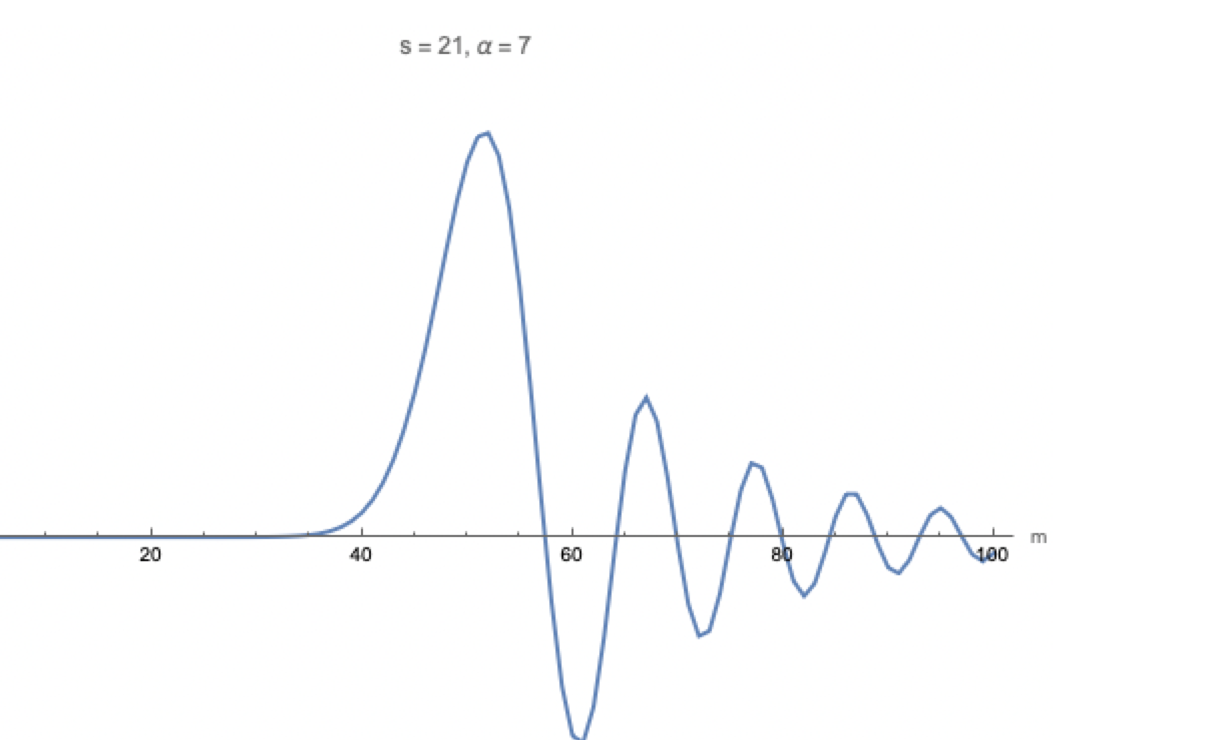
\includegraphics[width=0.82\linewidth]{../../notas-doctorado/imgs/wm_apachurrado_s21_alpha7.png}
  \caption{Distribuci\'on oscilatoria $W_m$ para un estado altamente apachurrado con $s=21$ y $\alpha=7$, como en el manuscrito.}
\end{figure}

\section{Evoluci\'on temporal de la funci\'on de Wigner}

Finalmente se analiza la evoluci\'on temporal de un estado apachurrado. La
funci\'on de Wigner inicial para $\alpha\in\mathbb R$ es
\begin{equation}
  W(x,p,0)
  =
  \frac{1}{\pi\hbar}
  \exp\left[
  -s(Kx-\sqrt2\alpha)^2
  -\frac{1}{s}\left(\frac{p}{\hbar K}\right)^2
  \right].
\end{equation}
Para un hamiltoniano arm\'onico,
\begin{equation}
  H=\frac{p^2}{2m}+\frac12m\omega^2x^2,
\end{equation}
las ecuaciones de Hamilton son
\begin{equation}
  \dot x=\frac{\partial H}{\partial p}=\frac{p}{m},
  \qquad
  \dot p=-\frac{\partial H}{\partial x}=-m\omega^2x.
\end{equation}
Combinando,
\begin{equation}
  \ddot x=\frac{1}{m}\dot p=-\omega^2x.
\end{equation}
Se propone la soluci\'on general
\begin{equation}
  x(t)=A\cos(\omega t)+B\sin(\omega t).
\end{equation}
Como
\begin{equation}
  p(t)=m\dot x(t)
  =
  m\omega[-A\sin(\omega t)+B\cos(\omega t)],
\end{equation}
las condiciones iniciales $x(0)=x_0$ y $p(0)=p_0$ dan
\begin{equation}
  A=x_0,
  \qquad
  p_0=m\omega B.
\end{equation}
Por tanto,
\begin{equation}
  x(t)=x_0\cos(\omega t)+\frac{p_0}{m\omega}\sin(\omega t),
\end{equation}
\begin{equation}
  p(t)=-m\omega x_0\sin(\omega t)+p_0\cos(\omega t).
\end{equation}
Usando
\begin{equation}
  K=\sqrt{\frac{m\omega}{\hbar}},
  \qquad
  m\omega=\hbar K^2,
\end{equation}
se escriben como
\begin{equation}
  x(t)=x_0\cos(\omega t)+\frac{p_0}{\hbar K^2}\sin(\omega t),
\end{equation}
\begin{equation}
  p(t)=-\hbar K^2x_0\sin(\omega t)+p_0\cos(\omega t).
\end{equation}

Para sustituir en la Wigner inicial, se necesitan las coordenadas iniciales
en funci\'on de las finales $x,p$. Es decir, se invierte la rotaci\'on
anterior. Del sistema se obtiene
\begin{equation}
  p_0=p\cos(\omega t)+\hbar K^2x\sin(\omega t),
\end{equation}
y
\begin{equation}
  x_0=x\cos(\omega t)-\frac{p}{\hbar K^2}\sin(\omega t).
\end{equation}
La Wigner evoluciona por composici\'on con el flujo cl\'asico:
\begin{equation}
  W(x,p,t)=W(x_0(x,p,t),p_0(x,p,t),0).
\end{equation}
Sustituyendo,
\begin{equation}
  \boxed{
  W(x,p,t)
  =
  \frac{1}{\pi\hbar}
  \exp\left\{
  -s\left[
  \cos(\omega t)Kx-\sin(\omega t)\frac{p}{\hbar K}
  -\sqrt2\alpha
  \right]^2
  -\frac{1}{s}\left[
  \sin(\omega t)Kx+\cos(\omega t)\frac{p}{\hbar K}
  \right]^2
  \right\}.
  }
\end{equation}
Esta expresi\'on muestra que la elipse de Wigner rota r\'igidamente en el
espacio fase con frecuencia $\omega$. El \'area de la elipse no cambia, pero
la direcci\'on apachurrada s\'i: en unos tiempos la incertidumbre reducida est\'a
principalmente en posici\'on, y en otros tiempos en momento.

\section{Comentario f\'isico}

Los estados apachurrados son esenciales en metrolog\'ia cu\'antica porque
permiten reducir el ruido en la cuadratura que se desea medir. El precio es
un aumento de ruido en la cuadratura conjugada. Esta redistribuci\'on no viola
Heisenberg; al contrario, es una manera controlada de usar la desigualdad de
incertidumbre. Por eso aparecen en interferometr\'ia, mediciones cu\'anticas no
destructivas y detectores como LIGO, donde la luz apachurrada permite reducir
el ruido de disparo en la cuadratura relevante.

\end{document}
